% ~ 6 pages
\chapter{Machine Learning}
\label{sec:ml}

\begin{itemize}
\item Supervised learning
\item Classification
\item Over-fitting
\end{itemize}

\section{Boosted Decision Trees}
\label{sec:bdt}

Keep this short!

Elements of statistical learning \cite{esl}

\begin{itemize}
\item Boosting: Adaptive Boosting $\alpha$, Gradient Boosting $\eta$
\item Node splitting: Gini Index
\item Hyperparameters: $N_\mathrm{Trees}$, $d_\mathrm{Tree}$,
\end{itemize}

\section{Neural Networks}
\label{sec:nn}

\subsection{Feedforward Neural Networks}
\label{sec:nn_feedforward}

\begin{figure}[ht]
  \begin{subfigure}[t]{0.55\textwidth}
    \centering
    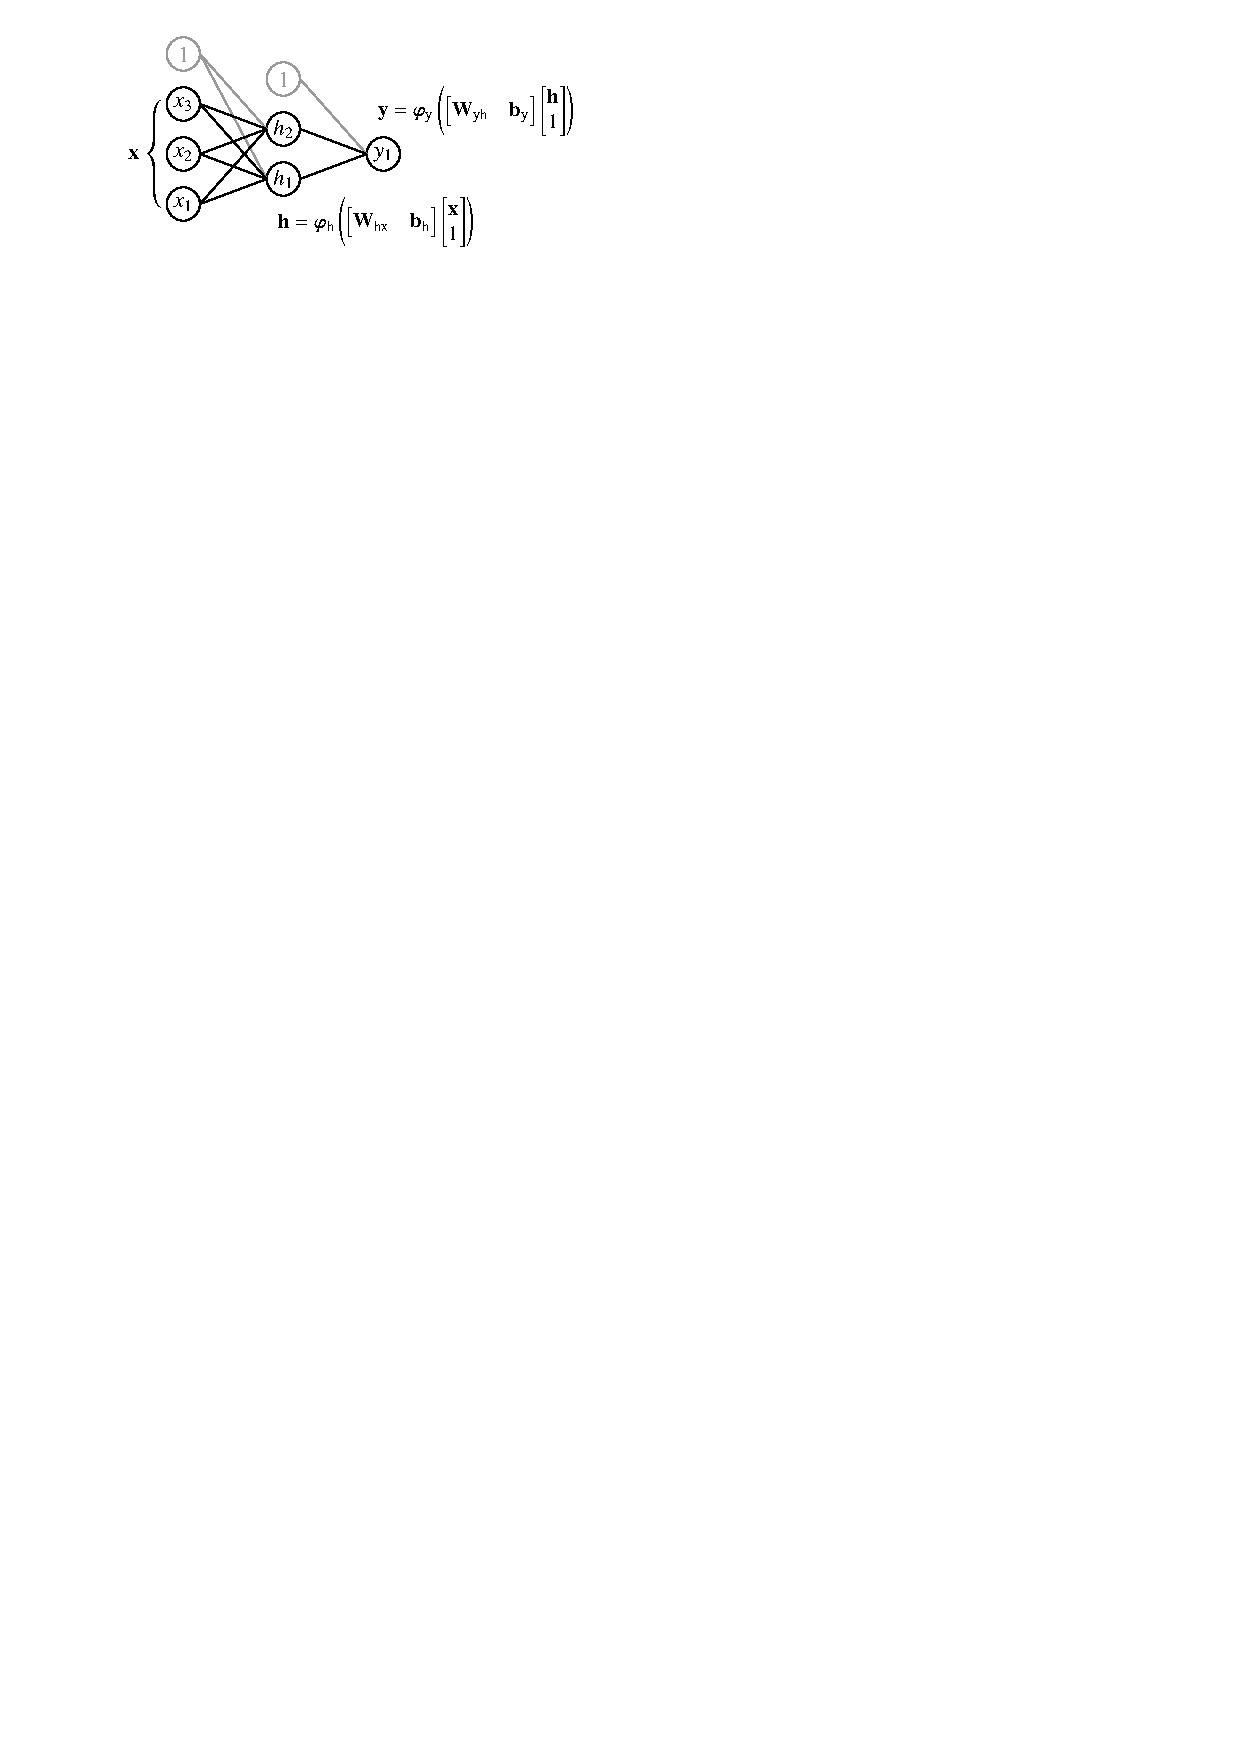
\includegraphics{./figures/theory/mlp.pdf}
    \subcaption{Schematic depiction of a multi-layer perceptron with input
      neurons $\mathbf{x}$, hidden layer activation $\mathbf{h}$ and output
      activation $\mathbf{y}$. The layers are connected via weight matrices
      $\mathbf{W}$ and optional bias vectors $\mathbf{b}$. Neuron activations
      are given after applying an element-wise activation function $\varphi$.}
    \label{fig:multi_layer_perceptron}
  \end{subfigure}\hfill
  \begin{subfigure}[t]{0.4\textwidth}
    \centering
    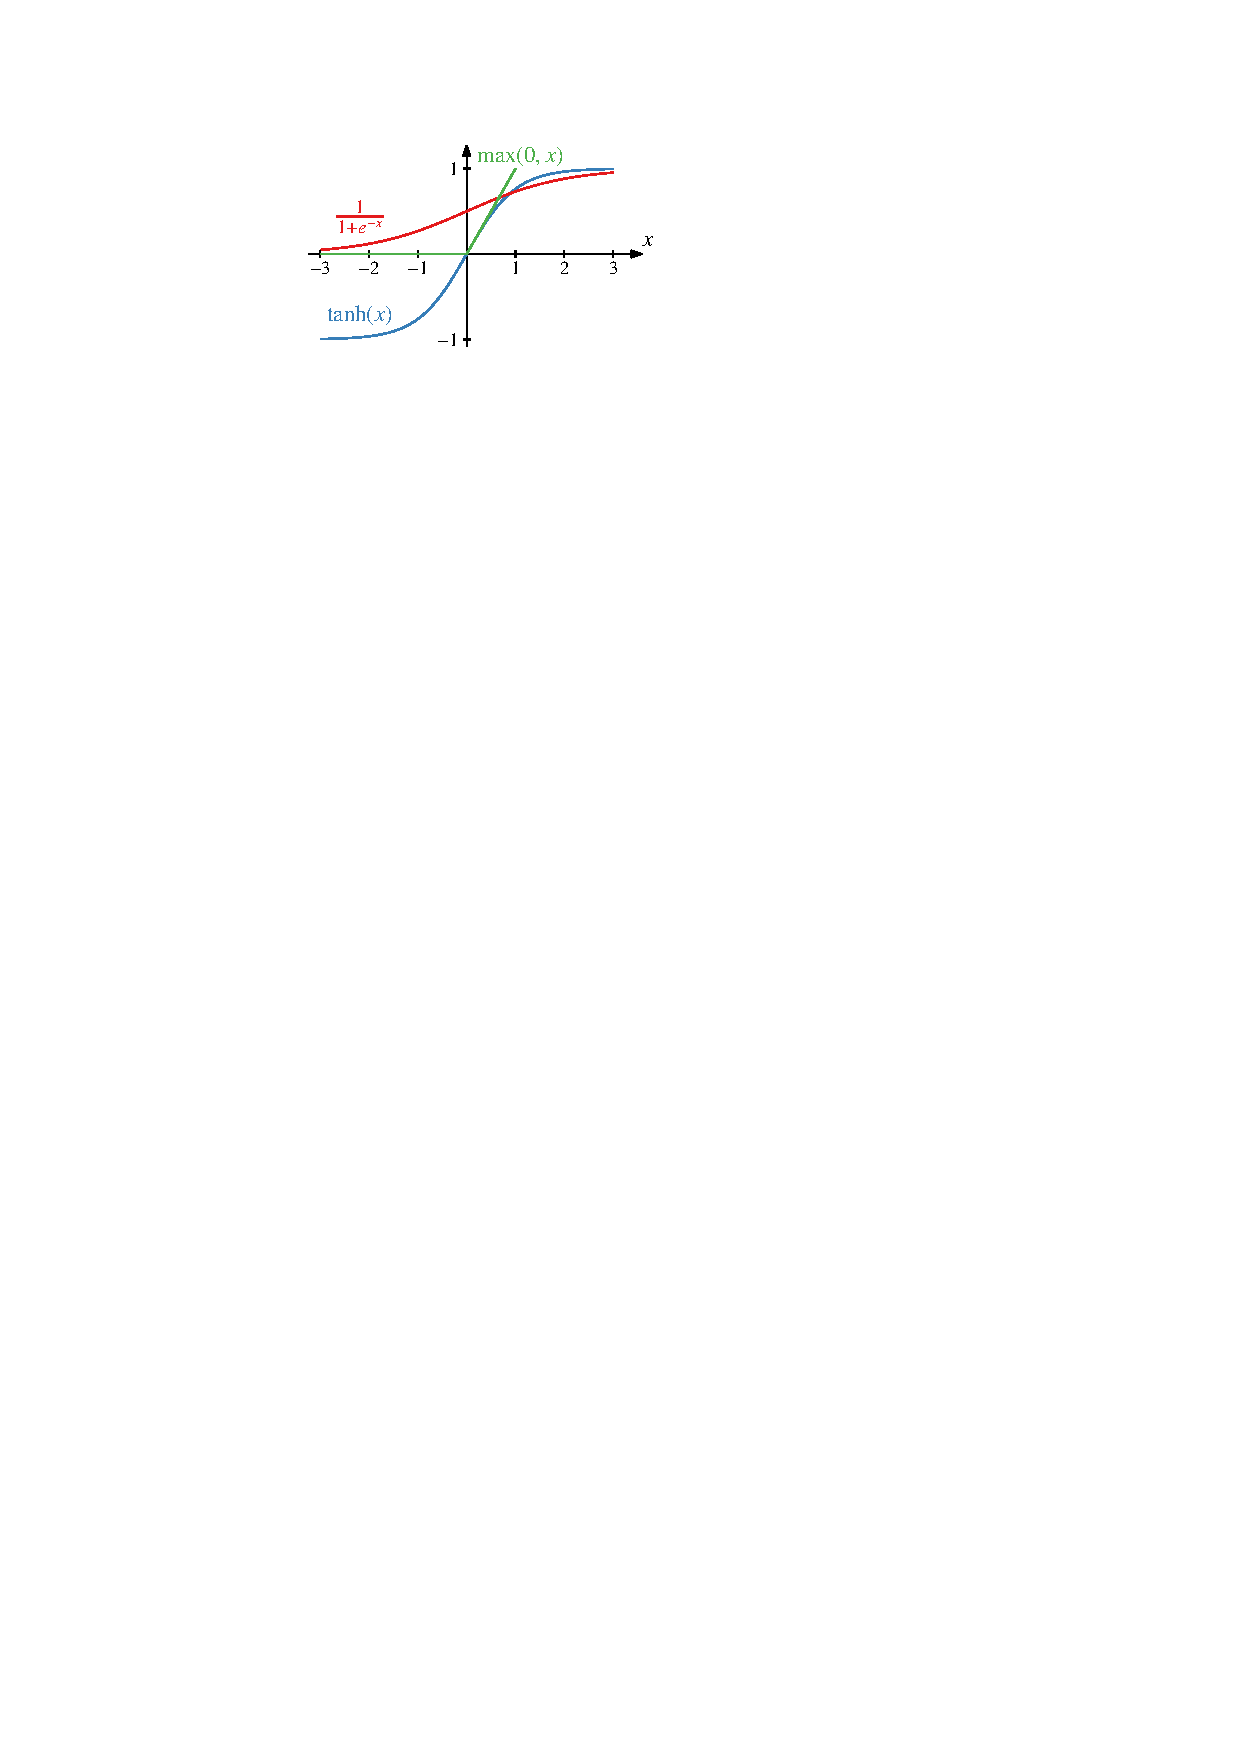
\includegraphics{./figures/theory/activation_functions.pdf}
    \subcaption{Commonly used activation functions for neural networks: logistic
      function (red), hyperbolic tangent (blue), and rectified linear unit --
      ReLU (green).}
    \label{fig:activation_functions}
  \end{subfigure}
  \caption{Feedforward neural network}
\end{figure}

Multi-layer perceptron (1 hidden layer):
\begin{align*}
  &\mathbf{h} = \varphi_{\text{h}}(\mathbf{W}_{\text{hx}} \mathbf{x} + \mathbf{b}_{\text{h}})
  &\mathbf{y} = \varphi_{\text{y}}(\mathbf{W}_{\text{yh}} \mathbf{h} + \mathbf{b}_{\text{y}})
\end{align*}
Layers are connected via linear transformations $W$ (and optionally biases $b$)
(affine transformations $W \, x + b$)
followed by a non-linear activation function $\varphi$. Layers connected in this
fashion are called densely-connected or dense layers. Layer sizes and activation
functions are hyperparameters of the model (except input and output layer which
is fixed by the underlying problem).

Typical activation functions are:
\begin{align}
  &\varphi_i(\mathbf{x}) = \frac{1}{1 + e^{-x_i}} &\text{Logistic / Sigmoid Function} \\
  &\varphi_i(\mathbf{x}) = \frac{e^{x_i}}{\sum_j e^{x_j}}&\text{Softmax}
                                                           \label{eq:softmax}
\end{align}
\cite{theano}

There are numerous different layers and ways to interconnect them, which allows
for high flexibility when building networks.

Training:
\begin{itemize}
\item Weight initialisation
\item Loss functions
\item Backpropagation \cite{lecun-backprop}
\item Mini-batch Gradient Descent
\item Cross-Validation
\end{itemize}

For the training of neural networks a loss function that penalises errors in the
model's predictions is needed. In $K$-class classification tasks a commonly used
loss function is the categorical cross-entropy. For an observation of true class
$k \in \{ 1, \dots, K \}$ with discriminants $\mathbf{x}$ and a model
$p(\mathbf{x})$ with per-class probabilities $p_k$ it is defined as
\begin{align*}
  L\left(k, p(\mathbf{x}) \right) = - \log\left( p_k(\mathbf{x}) \right) \eqdot
\end{align*}
For binary classification it is sufficient to give the predicted probability $p$
for the positive class (e.g.\ an observation being signal) such that the binary
cross-entropy can be written as
\begin{align*}
  L(p(\mathbf{x})) = -t \, \log(p(\mathbf{x})) - (1 - t) \, \log(1 - p(\mathbf{x})) \eqcomma
\end{align*}
where $t$ is the binary indicator of the true class (0 for the negative and 1
for the positive class). When looking at a subset of observations with event
weights $w_i$ the loss $\mathcal{L}$ is defined as
\begin{align*}
  \mathcal{L} = \frac{\sum_i w_i L_i}{\sum_j w_j} \eqcomma
\end{align*}
which in case of the cross-entropy can be interpreted as the negative
log-likelihood of the model parameters given the observed subset of data. These
losses expect networks to predict probabilities which can be met if the
activation function of the final layer is the logistic function or softmax (eq.
\ref{eq:softmax}). The training process minimises the loss $\mathcal{L}$
(maximises the likelihood) with respect to the model parameters, i.e.\ the
weights and biases of the network, given the observed training data.

\todo{Find proper references} \cite{esl}

Large penalties to predictions
that are far off. Its better to be sort of off instead of completely off.
Motivate where in this thesis these loss functions are used. Both losses are
also called 'Log Loss'. $p$ should be a class probability. Perfect classifiers
have loss of zero. Last layer in neural network effectively does logistic
regression on the intermediate representation created from the previous layers.

\section{Recurrent Neural Networks}
\label{sec:rnn}

Recurrent: If a network has one or more cycles, that is, if it is possible to
follow a path from a unit back to itself.

Physics motivation: Able to do regression and classification on sequences of
physics objects like tracks, clusters, particle flow objects etc..

\subsection{Fully-Connected RNN}
\label{sec:fully_connected_rnn}

% \textsc{Elman} network [Check Citation]\cite{elman}:
\textsc{Jordan} network \todo{look for citation}:
\begin{align*}
  \mathbf{c}_t &= \varphi_{\text{c}}\left( \mathbf{W}_{\text{c}} \mathbf{x}_{t} + \mathbf{U}_{\text{c}} \mathbf{h}_{t-1} + \mathbf{b}_{\text{c}} \right) \\
  \mathbf{h}_t &= \varphi_{\text{h}}\left( \mathbf{W}_{\text{h}} \mathbf{c}_{t} + \mathbf{b}_{\text{h}} \right)
\end{align*}
\todo{Should rename output $\mathbf{h}$ to $\mathbf{y}$ to be consistent.}
with trainable weights $\mathbf{W}$, recurrent weights $\mathbf{U}$ and biases $\mathbf{b}$.

Vanishing gradient problem: Applying the sigmoid function multiple times leads
to vanishing gradients (plot?).

\subsection{Long Short-Term Memory}
\label{sec:lstm}

\begin{figure}[t]
  \centering
  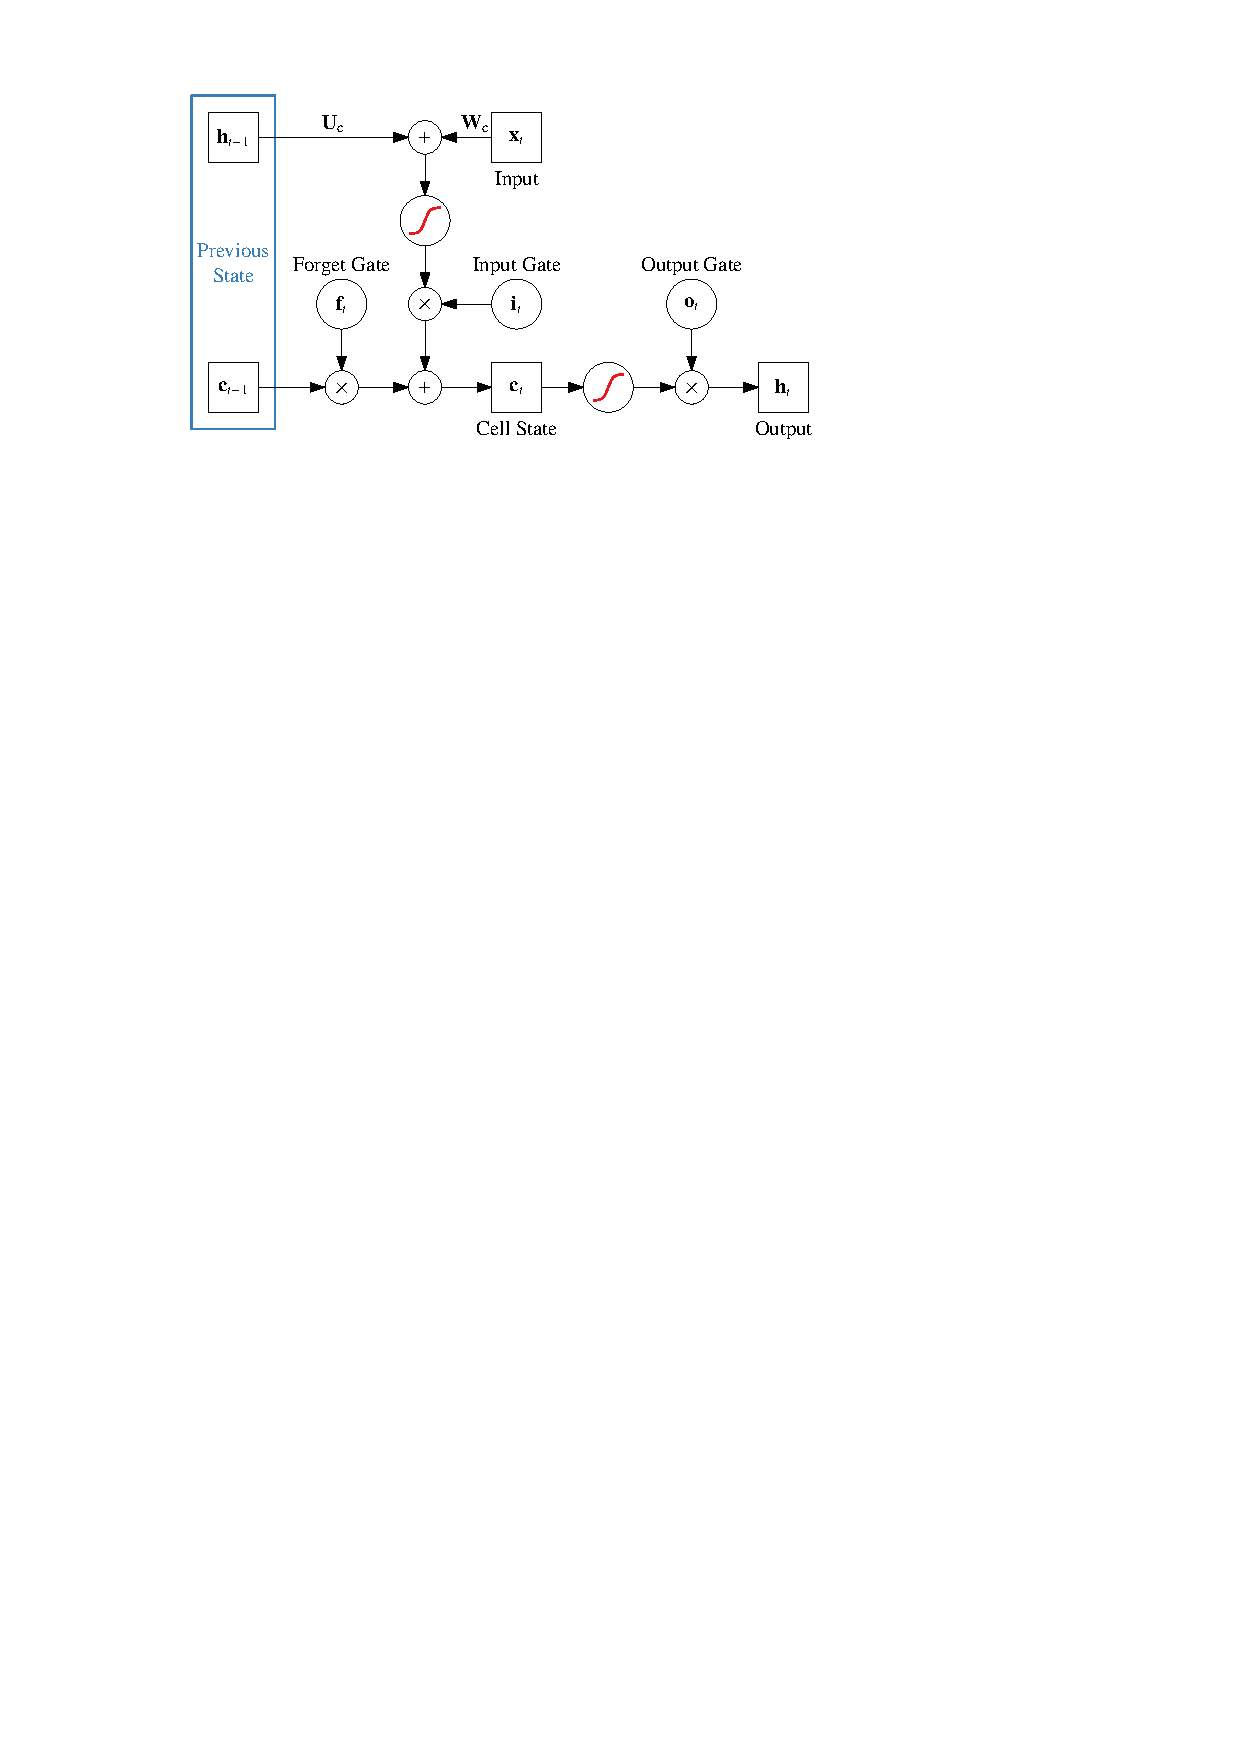
\includegraphics{./figures/theory/LSTM.pdf}
  \caption{Schematic description of a LSTM-cell.}
  \label{fig:schematic_lstm}
\end{figure}

[Check Citation]\cite{lstm}

Gate activations:
\begin{align*}
  \mathbf{f}_{t} &= \varphi_{\text{g}}\left( \mathbf{W}_{\text{f}} \mathbf{x}_{t} + \mathbf{U}_{\text{f}} \mathbf{h}_{t-1} + \mathbf{b}_{\text{f}} \right) &
  \mathbf{i}_{t} &= \varphi_{\text{g}}\left( \mathbf{W}_{\text{i}} \mathbf{x}_{t} + \mathbf{U}_{\text{i}} \mathbf{h}_{t-1} + \mathbf{b}_{\text{i}} \right) &
  \mathbf{o}_{t} &= \varphi_{\text{g}}\left( \mathbf{W}_{\text{o}} \mathbf{x}_{t} + \mathbf{U}_{\text{o}} \mathbf{h}_{t-1} + \mathbf{b}_{\text{o}} \right)
\end{align*}
Cell state update:
\begin{align*}
  \mathbf{c}_{t} &= \mathbf{f}_{t} \circ \mathbf{c}_{t-1}
                   + \mathbf{i}_{t} \circ \varphi_{\text{c}}(
                   \mathbf{W}_{\text{c}} \mathbf{x}_{t}+ \mathbf{U}_{\text{c}}
                   \mathbf{h}_{t-1} + \mathbf{b}_{\text{c}})
\end{align*}
Output:
\begin{align*}
  \mathbf{h}_{t} &= \mathbf{o}_{t} \circ \varphi_{\text{h}}(\mathbf{c}_{t})
\end{align*}

Stress that the gates depend on $x_t$ and $h_{t-1}$ via learn-able weights.
Therefore the inputting, outputting and forgetting is a learned process.

$\circ$: entry-wise product


Variables:
\begin{itemize}
\item $x_t$: input vector
\item $h_t$: output vector
\item $c_t$: cell state vector
\item $W$, $U$ and $b$: (recurrent -- $U$) weight matrices and bias vector
\item $f_t$, $i_t$ and $o_t$: gate vectors
  \begin{itemize}
  \item $f_t$: forget gate vector
  \item $i_t$: input gate vector
  \item $o_t$: output gate vector
  \end{itemize}
\end{itemize}

Activation functions:
\begin{itemize}
\item $\sigma_g$: element-wise sigmoid function (Gate activation -- recurrent
  activation)
\item $\sigma_c$: element-wise hyperbolic tangent (Cell activation -- recurrent
  activation)
\item $\sigma_h$: element-wise hyperbolic tangent (Output activation)
\end{itemize}


\section{Technical Setup}
\label{sec:tech_setup}

Frameworks used for this thesis (theano \cite{theano}, keras \cite{keras})

Optimiser: Adam

Masking layer


%%% Local Variables:
%%% mode: latex
%%% TeX-master: "mythesis"
%%% End:
